\documentclass[serif,mathserif]{beamer}
\usepackage{amsmath, amsfonts, epsfig, xspace}
\usepackage{algorithm,algorithmic}
\usepackage{pstricks,pst-node}
\usepackage{multimedia}
\usepackage[normal,tight,center]{subfigure}
\setlength{\subfigcapskip}{-.5em}
\usepackage{beamerthemesplit}
\usetheme{keynote}

%----------Hacks-----------------
%http://www.shawnlankton.com/2008/02/beamer-and-latex-with-keynote-theme/
%\titlegraphic{\includegraphics[height=1cm]{your_logo.png}}
%\pgfdeclareimage[height=0.5cm]{iwmi-logo}{iwmi1}
%\logo{\pgfuseimage{iwmi-logo}}
\setbeamercolor{titlelike}{parent=structure,fg=white}
%-----------------------------------

\author[NCO]{Niroshan Bandara \quad Nishadi Eriyagama\\Lal Muthuwatta \quad Nirosha Liyanage\\ Yann Chemin }

\title[IWMI\hspace{2em}\insertframenumber/\inserttotalframenumber]{A National Climate Observatory\\for Sri Lanka}

\date{November 11, 2014} %leave out for today's date to be insterted

\institute{IWMI}

\begin{document}

\maketitle
\Large
% \section{Introduction}  % add these to see outline in slides

%\begin{frame}
%  \frametitle{CGIAR}
%
%Consultative Group for International Agricultural Research\\
%Ratified on October 2nd, 2013\\
%Full Open Access \& Open Source\\
%Research data and publication
%\begin{columns}
%\column{0.5\textwidth}
%\begin{center}
%\begin{itemize}
% \item International Public Goods
% \item Public Domain
% \item Publications Open Access
% \item FOSS models and algorithms
%\end{itemize}
%\end{center}
%
%\column{0.5\textwidth}
%\begin{center}
%  \includegraphics[width=1.5cm]{CGIAR_Green}
%  \hspace{5mm}
%  \includegraphics[width=2cm]{WLE_and_partners-vertical_logo_strip.png}
%\end{center}
%\end{columns}
%\vspace{2mm} 2018: all 15 CG centres, already FOSS4G Lab:
%(\href{http://gsl.worldagroforestry.org}{gsl.worldagroforestry.org})
%\end{frame}

\transdissolve<5>
% \section{Main Body} % add these to see outline in slides

%/ Sri Lanka floods hit over 500 thousand people. At least 52 dead and 8 missing. At least 503,406 people from 137,019 families have been affected by monsoon floods and landslides in Sri Lanka over the past month. According to data from the Meteorology Department and Disaster Management Centre (DMC), more than 5,370 houses were destroyed while 33,571 were partially damaged. So far, the death toll stands at 52 dead and eight missing. /
%
%/ "Although Sri Lanka is geographically situated to endure frequent flooding, this is the worst in eight years," said GFA president K P Yohannan. christiantoday.com /

\begin{frame}
  \frametitle{Sri Lankan Climate is changing}
\begin{columns}
\column{0.7\textwidth}
\begin{center}
\begin{itemize}
 \item Droughts Damage Agriculture
 \item High Rainfall Brings Floods
 \item Lanslides Are Increasing
\end{itemize}
\end{center}

\column{0.3\textwidth}
\begin{center}
   \includegraphics[width=3.5cm]{sri-lanka-flood1}
   \vspace{2mm}
\end{center}
\end{columns}
\includegraphics[width=8cm]{20120812_Polonnaruwa-Prakramasamudrya}
\end{frame}

\transdissolve<5>

\begin{frame}
 %\frametitle{What is needed?}
\begin{center}
We need to know the weather now\\
\ \\
publicly available\\
\ \\
real-time\\
\ \\
from local sources
\end{center}
\end{frame}

\transdissolve<5>

\begin{frame}
  \frametitle{Why do we need this?}
  \begin{center}
  \includegraphics[height=6.5cm]{Screenshot_2014-10-22-15-05-21}
  \hspace{1mm}
  \includegraphics[height=6.5cm]{IMG_20141022_150543}
  \end{center}
\end{frame}

\transdissolve<5>

\begin{frame}
  \frametitle{A National Climate Observatory}
\begin{columns}
\column{0.6\textwidth}
\begin{center}
\begin{itemize}
 \item National grid of stations
 \item Land and sea
 \item Public website
 \item Mobile Apps
\end{itemize}
\end{center}

\column{0.4\textwidth}
\begin{center}
 \includegraphics[width=4.5cm]{ws500.png}
\end{center}
\end{columns}
\end{frame}

\transdissolve<5>

\begin{frame}
  \frametitle{National grid of stations}
\begin{columns}
\column{0.6\textwidth}
\begin{center}
\begin{itemize}
 \item 500 Weather Stations
 \item 5 minutes Reporting
 \item Climate-Based Grid
 \item Online
 \item 1/20$^{th}$ Cost 
 \item Improve Forecasting
\end{itemize}
\end{center}

\column{0.4\textwidth}
\begin{center}
 \includegraphics[width=4.5cm]{ws500.png}
\end{center}
\end{columns}
 \vspace{1mm}
\end{frame}

\transdissolve<5>

\begin{frame}
  \frametitle{Land and Seas}
\begin{columns}
\column{0.5\textwidth}
\begin{center}
\begin{itemize}
 \item Land systems
 \item Buoys at sea
\end{itemize}
\end{center}

\column{0.5\textwidth}
\begin{center}
 \includegraphics[width=5cm]{Sri-Lanka-Navy-Divers-Place-Buoys-in-Back-Bay}
\end{center}
\end{columns}
 \includegraphics[width=5cm]{dart-buoy-ndbc-03-30-2006}
\end{frame}

\transdissolve<5>

\begin{frame}
  \frametitle{Data}
\begin{columns}
\column{0.5\textwidth}
\begin{center}
\begin{itemize}
 \item Wind
 \item Rainfall
 \item Temperature
\end{itemize}
\end{center}

\column{0.5\textwidth}
\begin{center}
\begin{itemize}
 \item 10+ other records
 \item Sea Roughness 
 \item Sea Temperature
\end{itemize}
\end{center}
\end{columns}
\vspace{2mm}
\begin{center}
 \includegraphics[width=10.5cm]{rain_record}
\end{center}
\end{frame}

\transdissolve<5>

\begin{frame}
  \frametitle{Website}
  \begin{center}
  \includegraphics[height=4.5cm]{wu_banner}
  \hspace{1mm}
  \includegraphics[height=4.5cm]{wundergound}
  \end{center}
\end{frame}
%\begin{frame}
%  \frametitle{Equations}
%  Equations are easy
%  \begin{itemize}
%  \item Just and paste equations\pause
%  \item From the paper!
%    \begin{equation*}
%      \textbf{p}^* = \underset{\textbf{p}}{\arg\!\min}~\sum_{\textbf{x}}\left[ I(\textbf{W}(\textbf{x};\textbf{p})) - T(\textbf{x}) \right]^2
%    \end{equation*}
%  \end{itemize}
%\end{frame}

\transdissolve<5>

\begin{frame}
  \frametitle{Mobile Apps}
  \begin{figure}[t]
    \centering
    \includegraphics[height=4.5cm]{mobileApp4}
    \hspace{1mm}
    \includegraphics[height=4.5cm]{Screenshot_2014-10-17-23-57-13}
  \end{figure}
\end{frame}

\transdissolve<5>

\begin{frame}
  \frametitle{Warning Systems}

\begin{columns}
\column{0.4\textwidth}
\begin{itemize}
\item SMS
\item Tsunami
\item News Alerts
\item Voice call
\end{itemize}

\column{0.6\textwidth}
\begin{center}
    \includegraphics[height=3.5cm]{Mobile_woman_image-from-teleusebop-film}
\end{center}
\end{columns}
\end{frame}

\transdissolve<5>

\begin{frame}
  %\frametitle{Benefits}
  \begin{center}
  \Huge{Benefits}
  \end{center}
\end{frame}

\transdissolve<5>

\begin{frame}
  \frametitle{Disaster Warning}
\begin{columns}
\column{0.5\textwidth}
\begin{center}
\Large{
\begin{itemize}
 \item Floods
 \item Landslides
 \item Droughts
 \item Hurricanes
 \item Rough Sea
\end{itemize}
}
\end{center}

\column{0.5\textwidth}
\begin{center}
 \includegraphics[width=3.5cm]{floods1}
 \vspace{1mm}
 \includegraphics[width=3.5cm]{Drought-hits-North-of-Sri-Lanka-}
\end{center}
\end{columns}
\end{frame}

\transdissolve<5>
%Spilling Upper Kotmale Dam
%http://rmthilina.blogspot.com/2012/08/iet-sri-lanka-field-visit-to-upper.html
\begin{frame}
  \frametitle{Energy}
\begin{columns}
\column{0.65\textwidth}
\begin{center}
\Large{
\begin{itemize}
 \item Hydro Power Maximization
 \item Wind Farm Zoning
 \item Solar Power Zoning
\end{itemize}
}
\end{center}

\column{0.35\textwidth}
\begin{center}
 \includegraphics[width=4.1cm]{spilling_upper_Kotmale_Dam}
\end{center}
\end{columns}
\vspace{5mm}
\begin{center}
\includegraphics[height=2.5cm]{solar-panels-of-the-first-solar-power-plant-of-sl}
\hspace{5mm}
\includegraphics[height=2.5cm]{Seguwantivu_and_Vidatamunai_Wind_Farms5_1}
\end{center}
\end{frame}

\transdissolve<5>
%Paddy photo
%http://ourinheritancesl.blogspot.com/2013/04/paddy-cultivation-in-sri-lanka-part-2.html
\begin{frame}
  \frametitle{Agriculture}
\begin{columns}
\column{0.95\textwidth}
\begin{center}
\begin{itemize}
 \item Droughts Warning
 \item Production Improvement 
 \item Irrigation/Reservoir Services Optimization
\end{itemize}
\end{center}

\column{0.05\textwidth}
\end{columns}
\vspace{5mm}
\begin{center}
 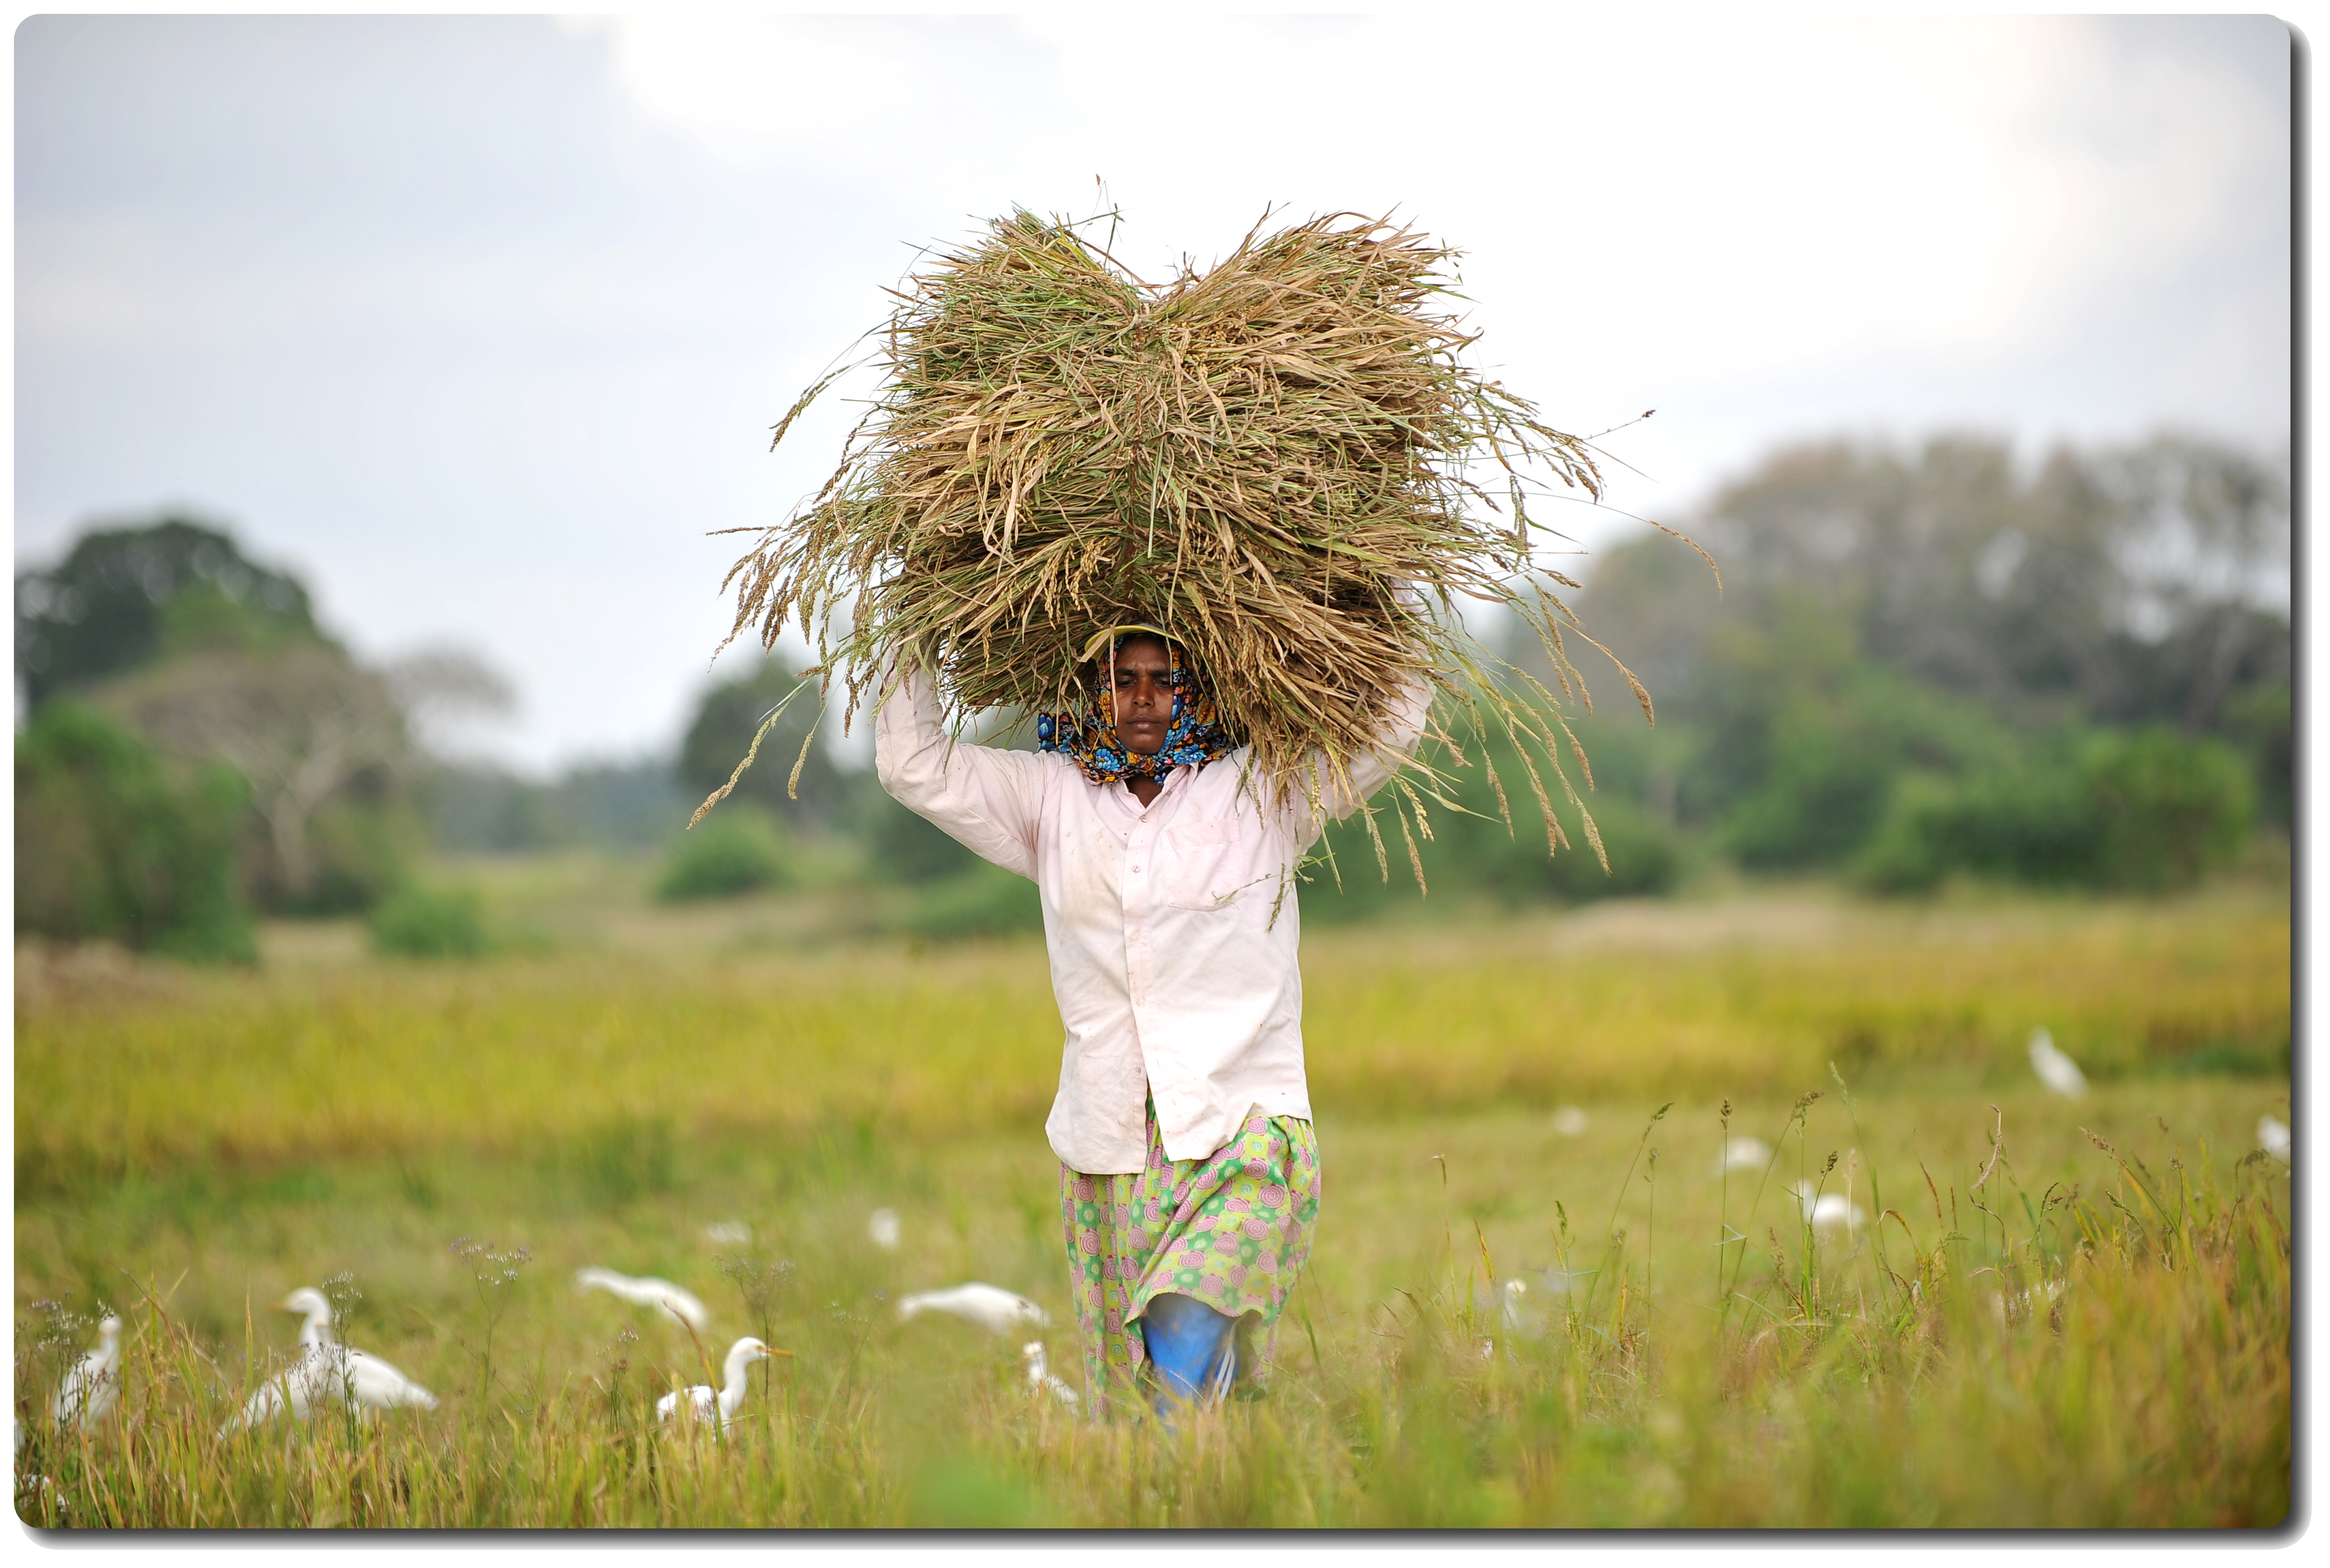
\includegraphics[height=3.25cm]{fromNeil/NPRiceHarvest}
 \hspace{2mm}
 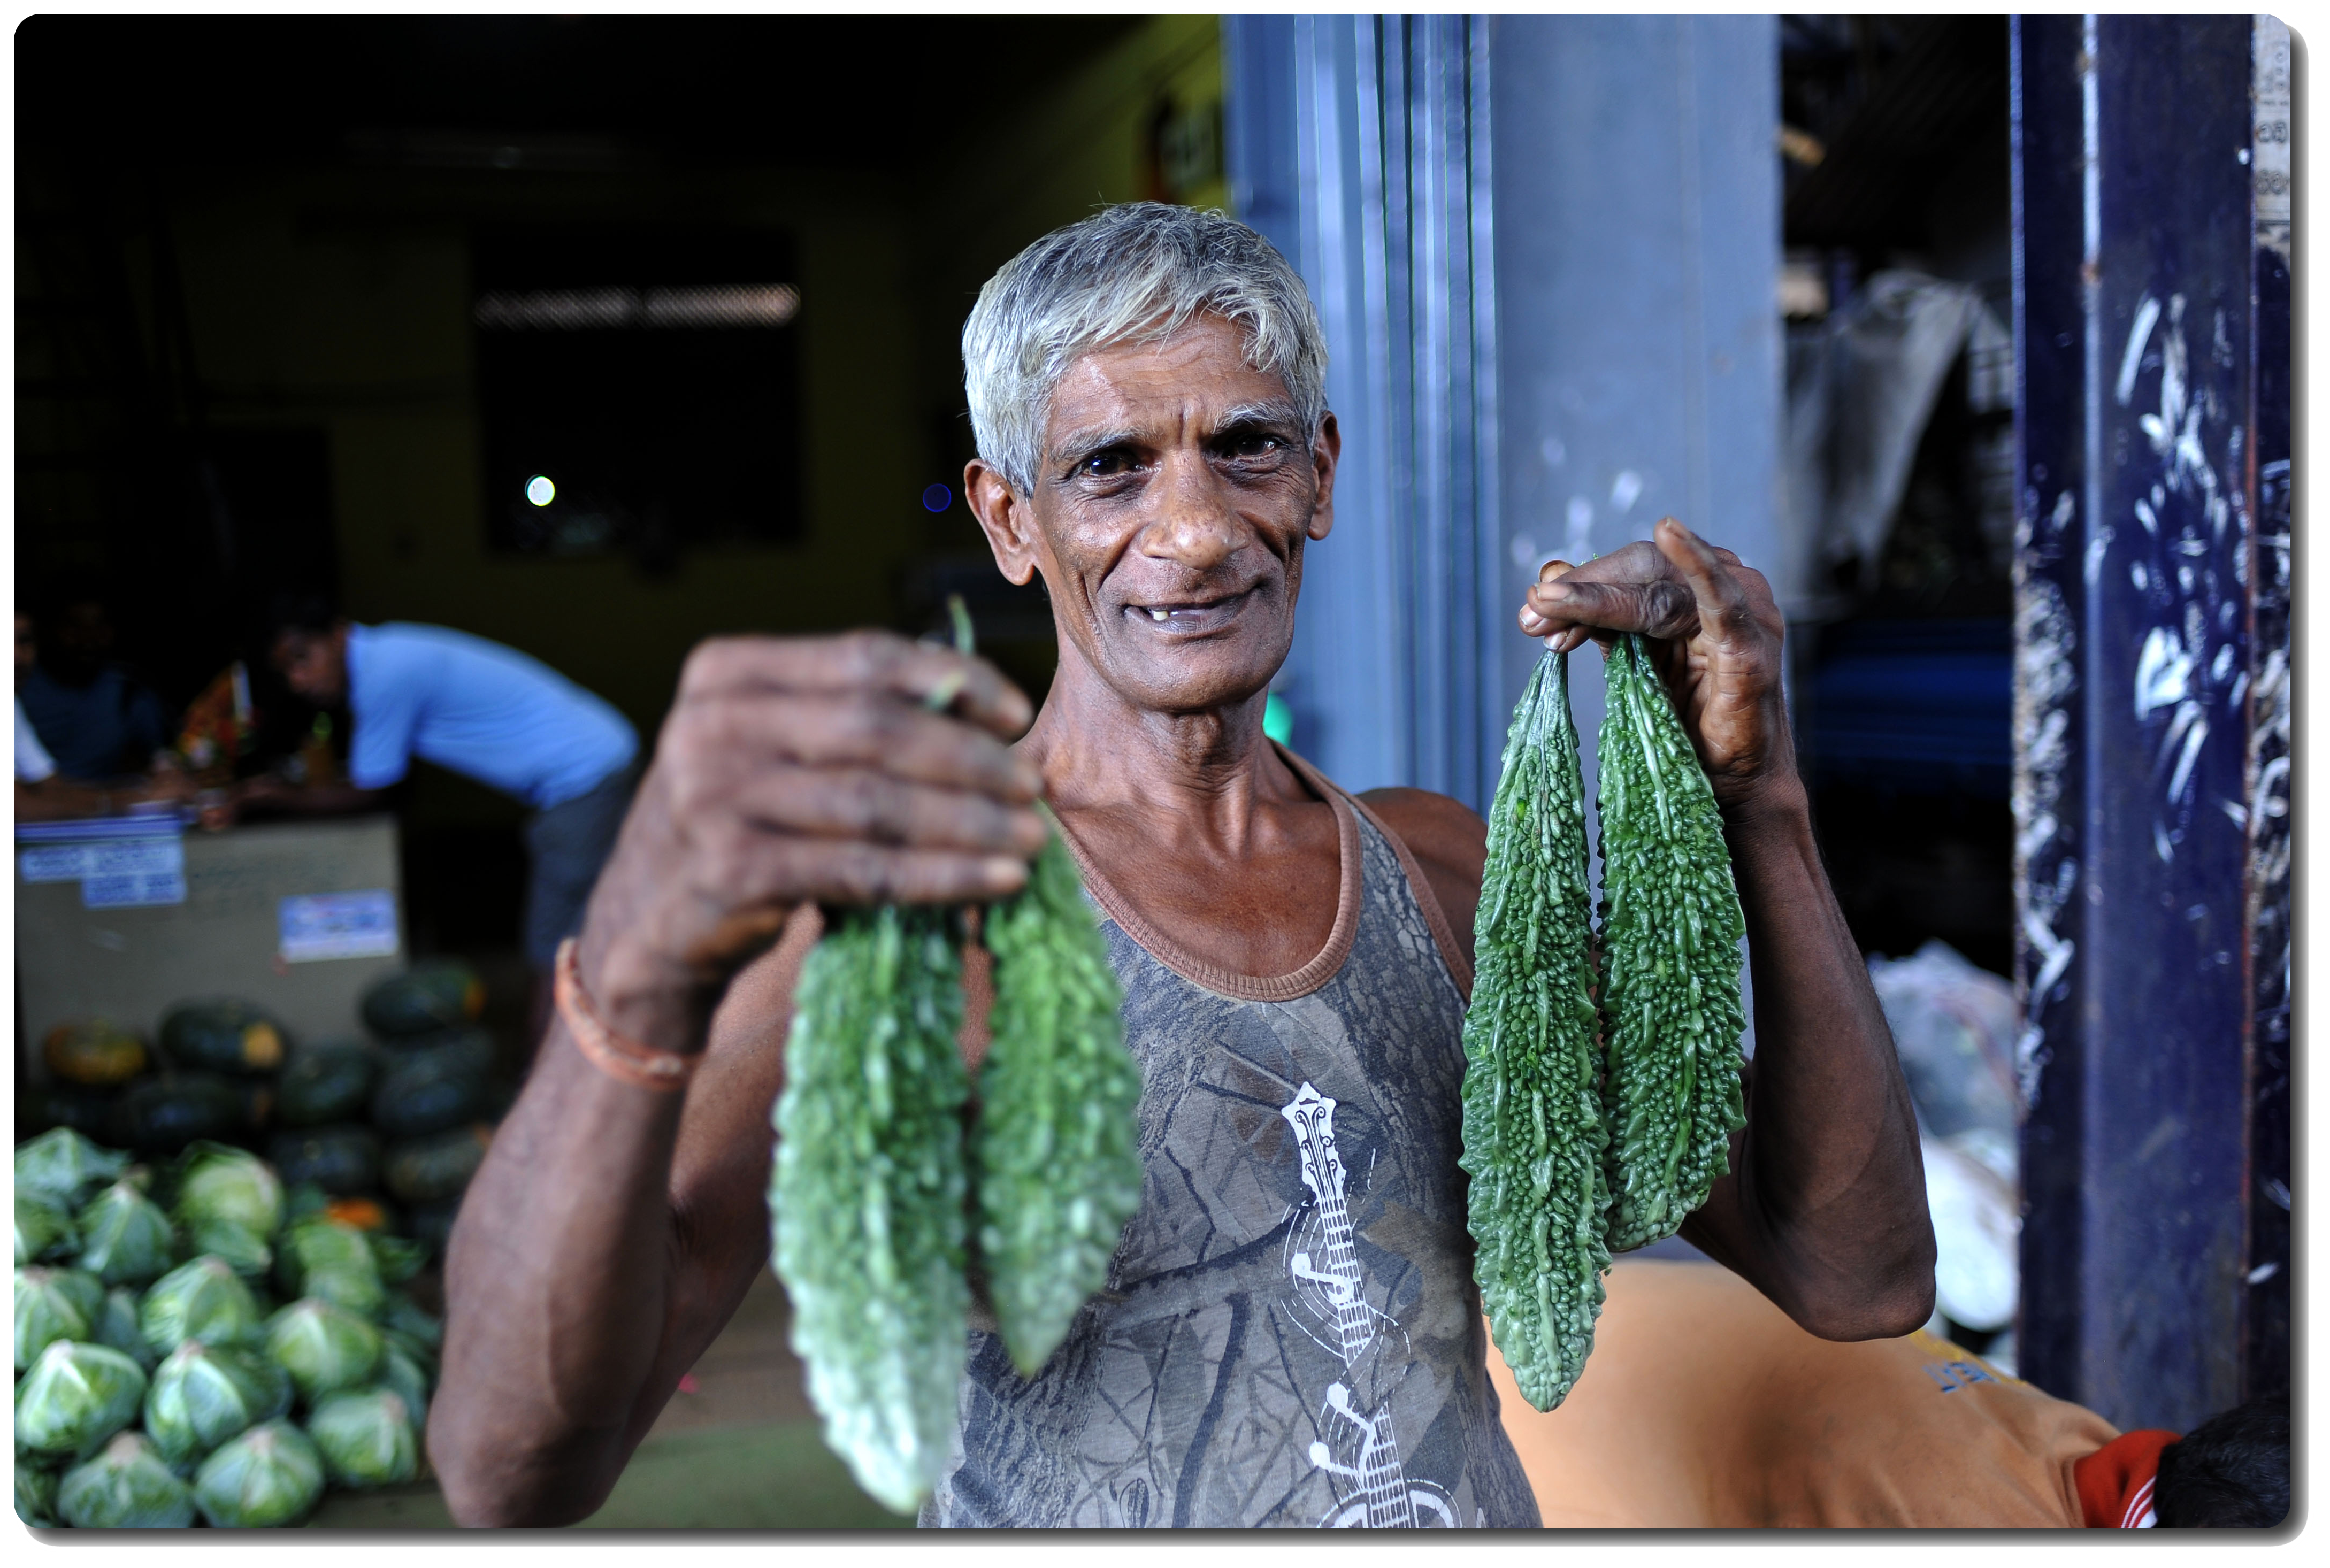
\includegraphics[height=3.25cm]{fromNeil/NP-Dambula}
\end{center}
\end{frame}

\transdissolve<5>
%Paddy photo
%http://ourinheritancesl.blogspot.com/2013/04/paddy-cultivation-in-sri-lanka-part-2.html
\begin{frame}
  \frametitle{Plantations}
\begin{columns}
\column{0.8\textwidth}
\begin{center}
\begin{itemize}
 \item Close Monitoring of Production
 \item Production Improvement Support
\end{itemize}
\end{center}
\column{0.3\textwidth}
\begin{flushleft}
 \hspace{3.5mm}
 \includegraphics[width=2cm]{thambili}
\end{flushleft}
\end{columns}
\begin{center}
 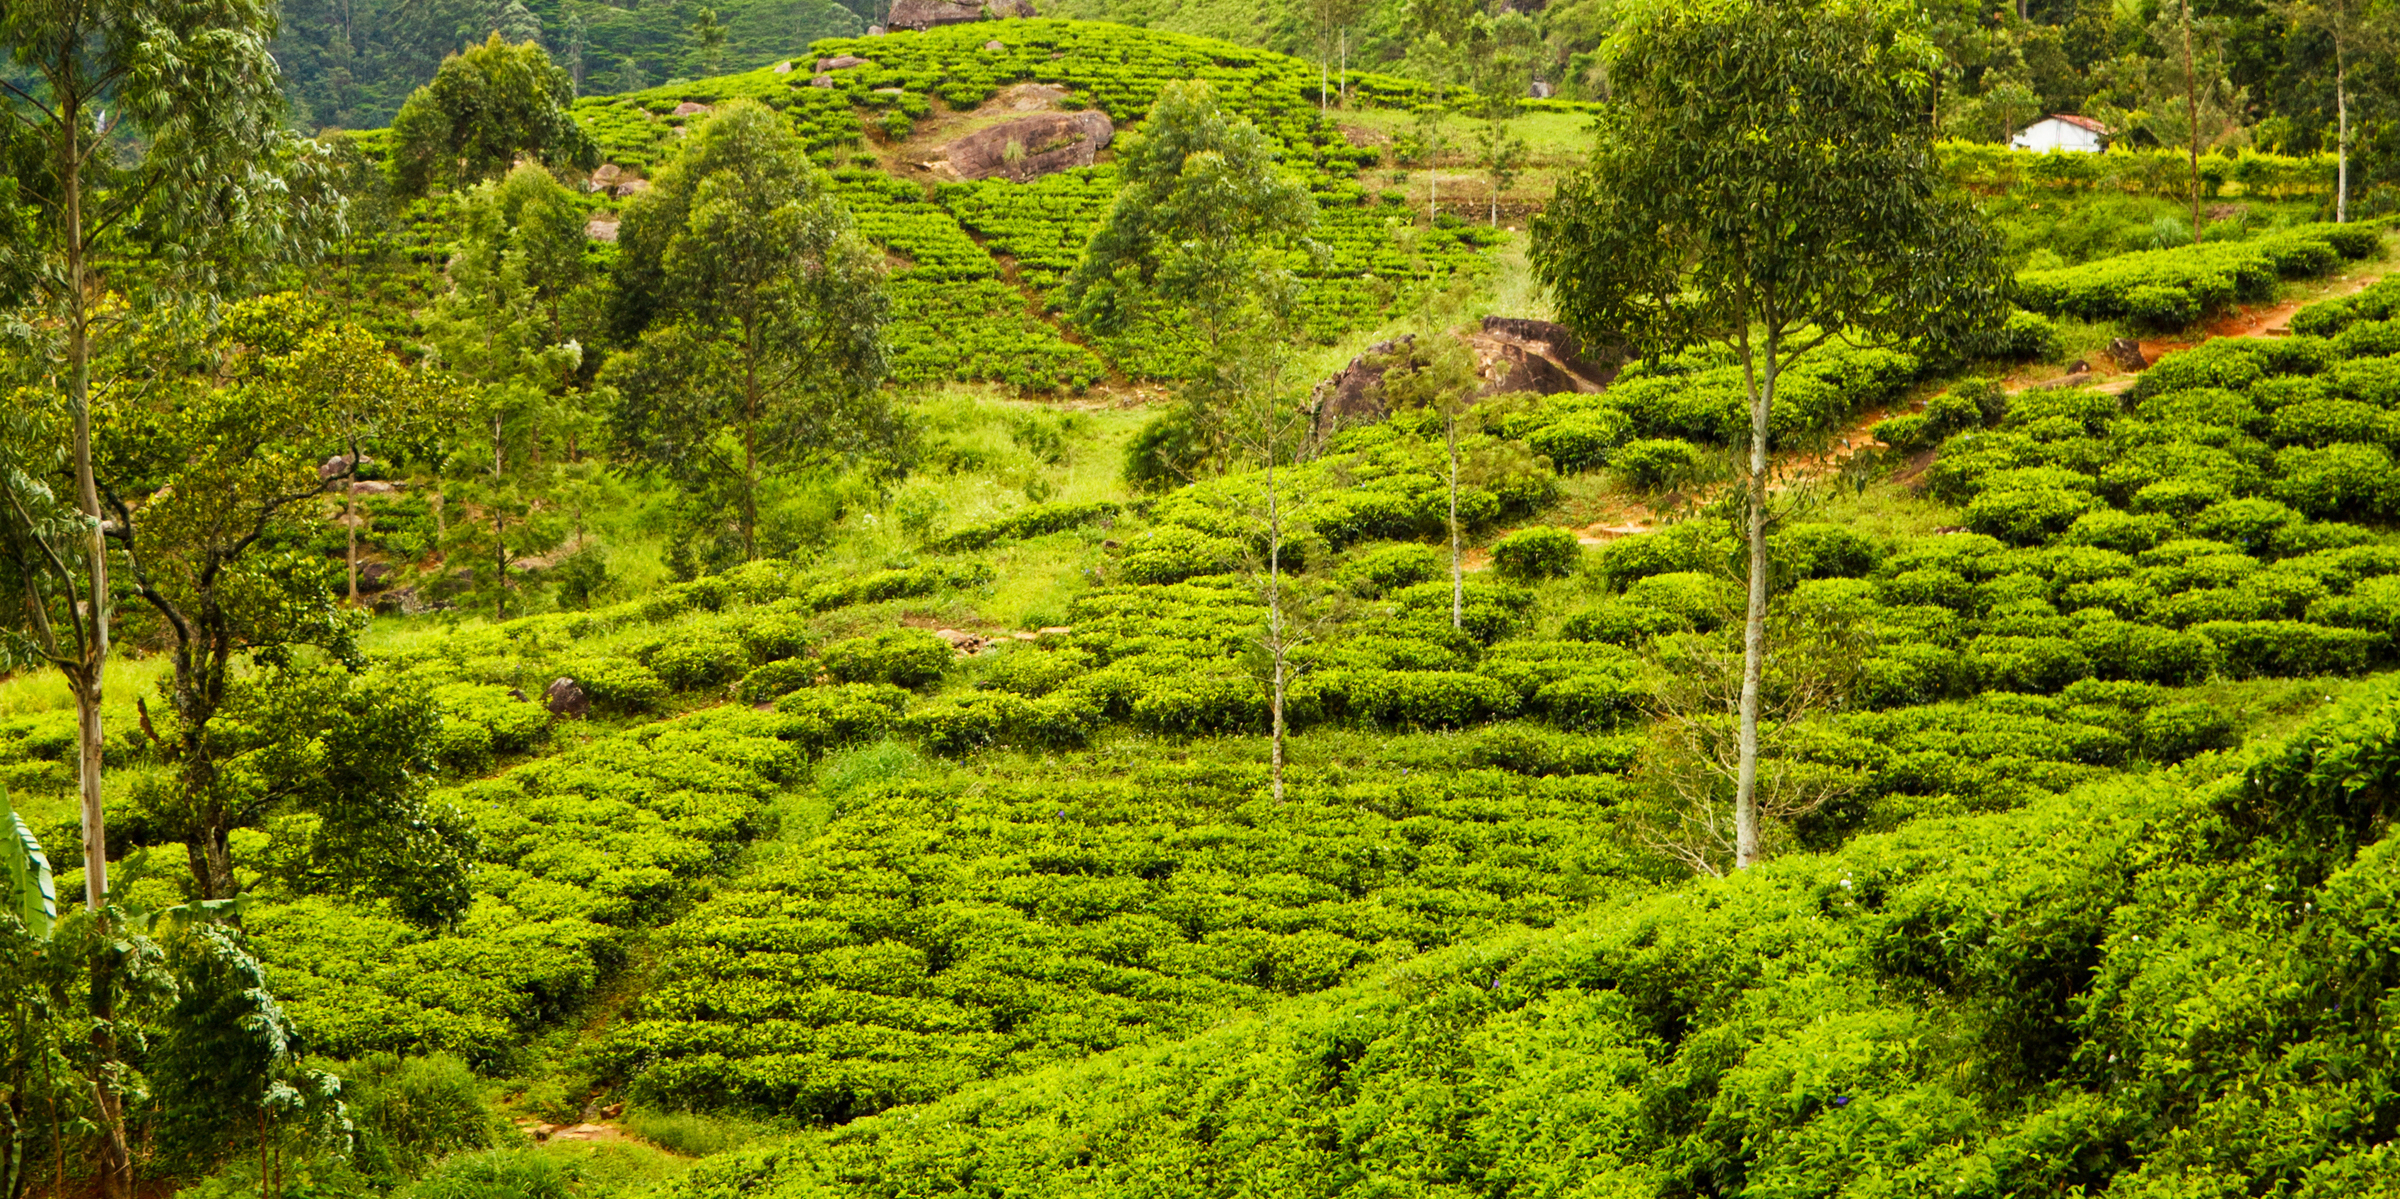
\includegraphics[height=3cm]{sri_lanka_tea_plantation}
 \hspace{5mm}
 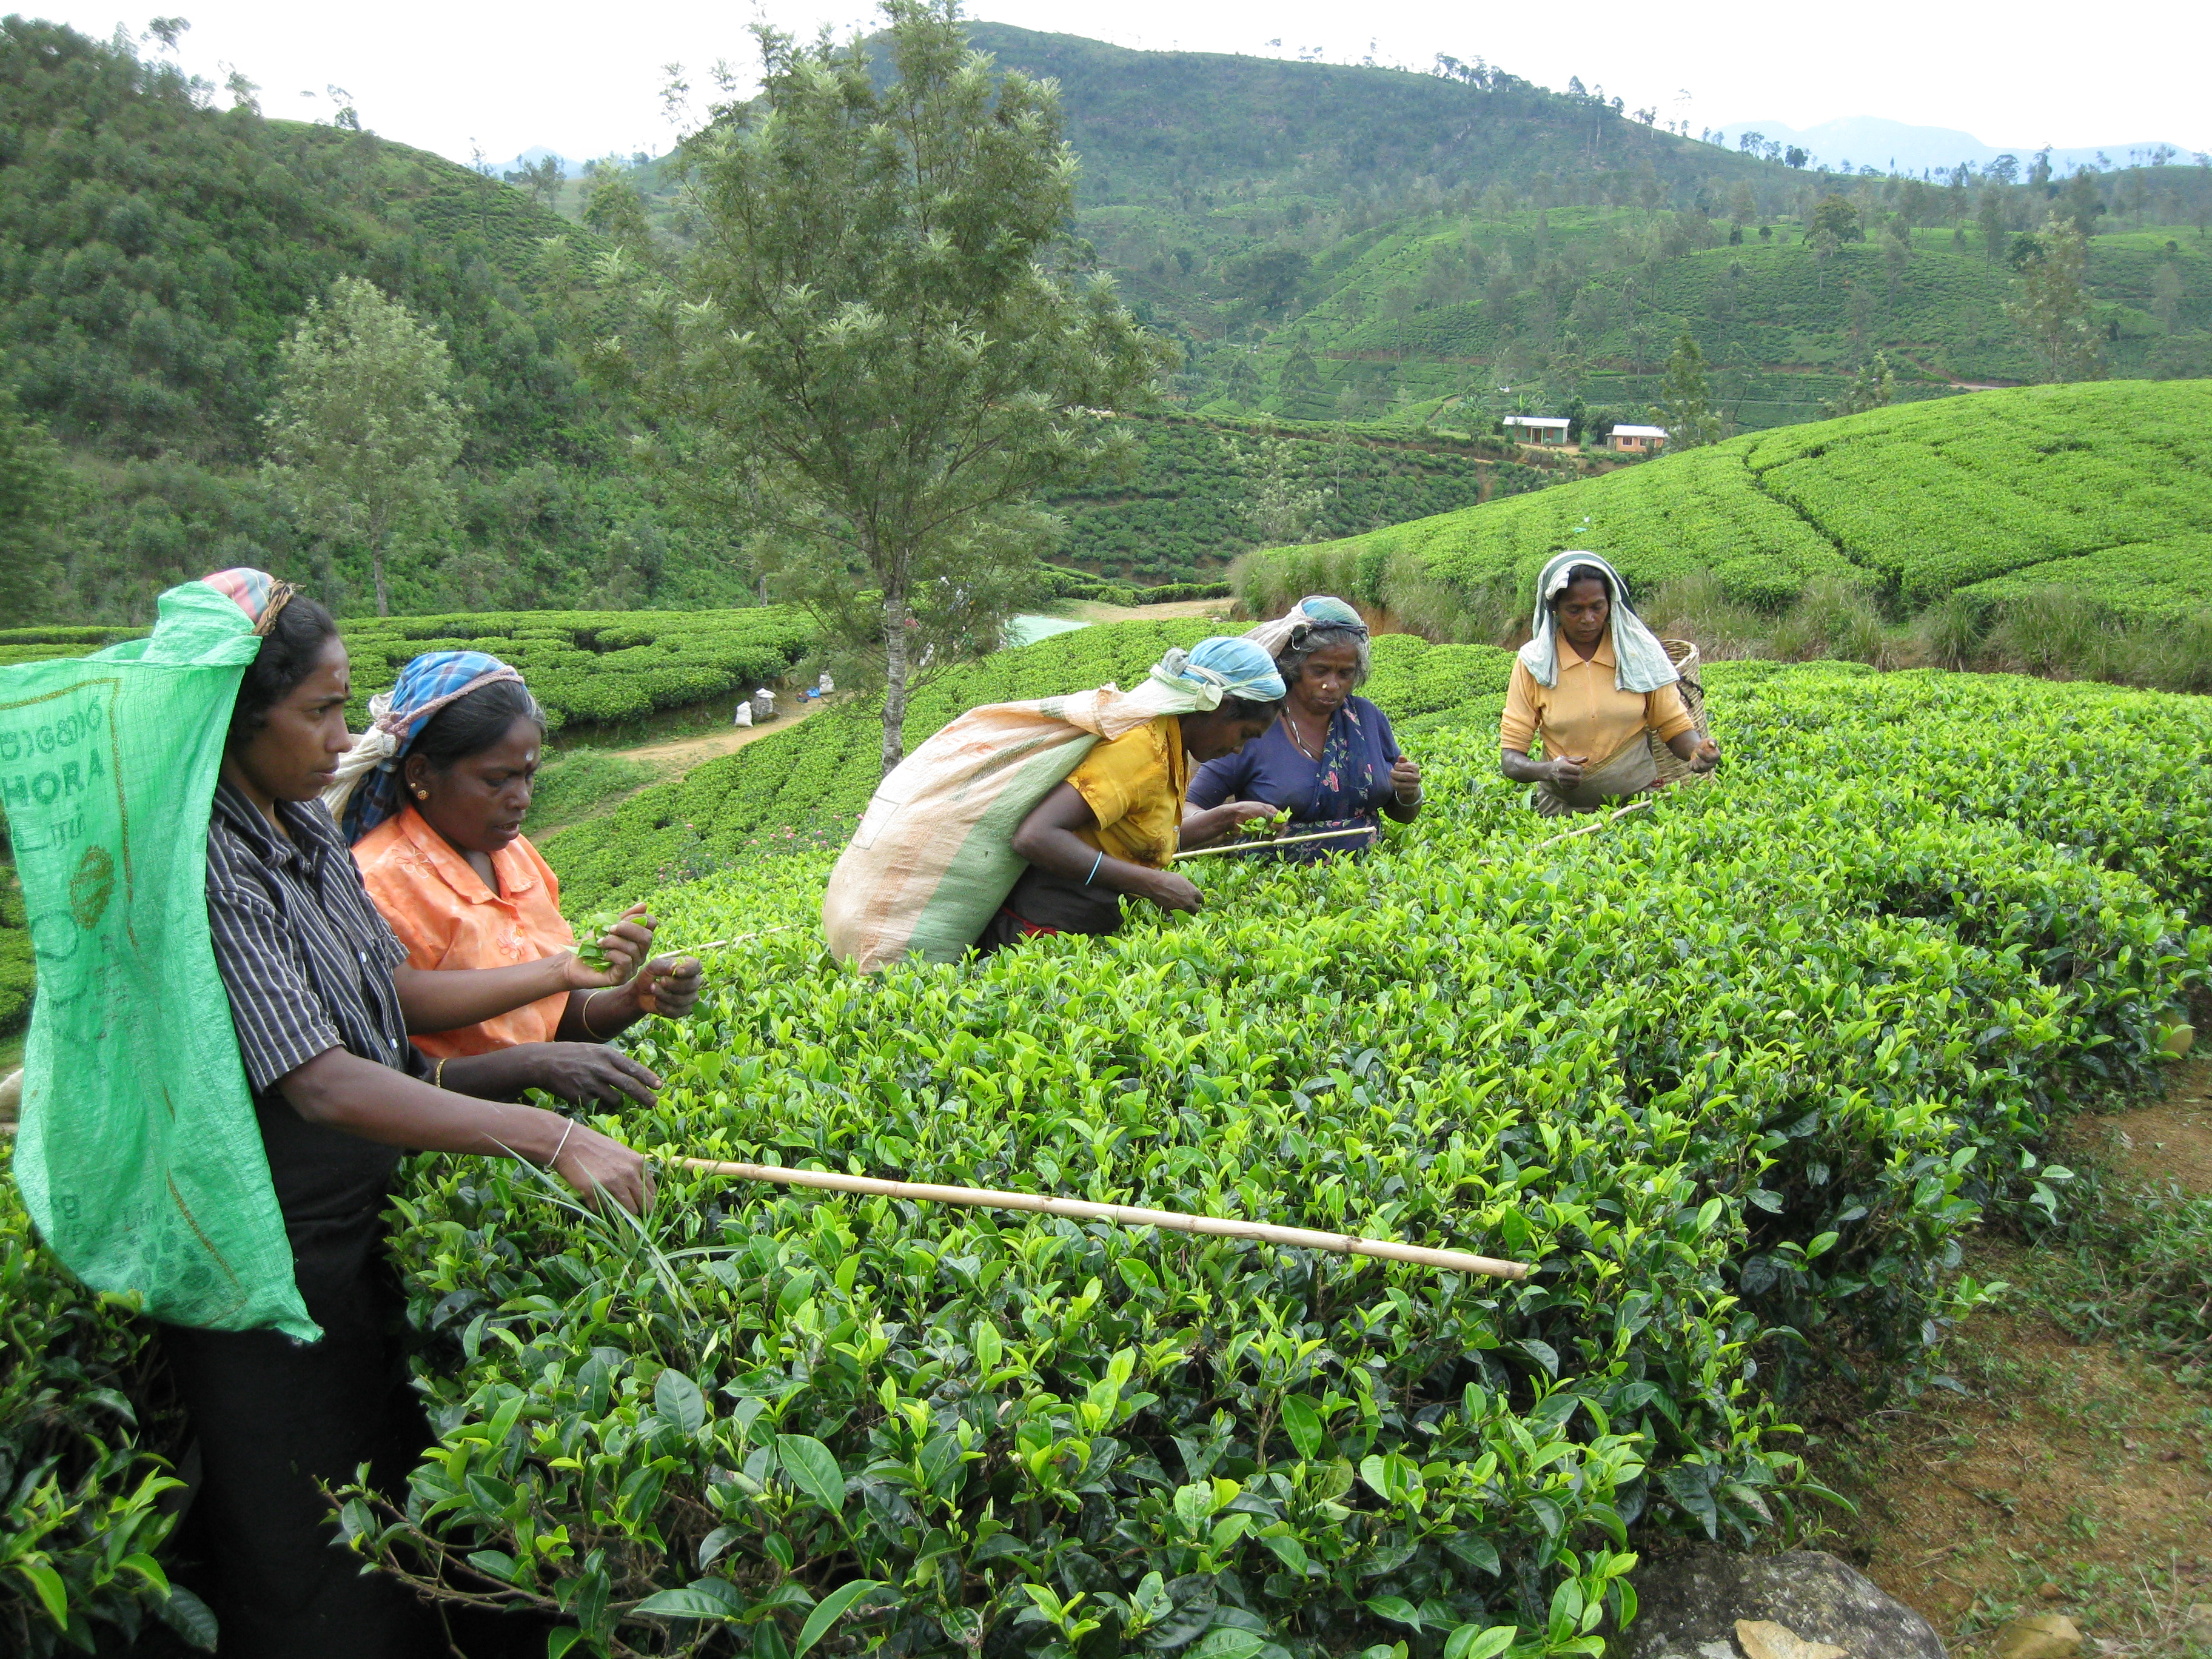
\includegraphics[height=3cm]{Sri-Lanka532}
\end{center}
\end{frame}

\transdissolve<5>
%Tsunami buoys
%http://www.noaanews.noaa.gov/stories2006/s2749.htm
%Boat capsized
%http://newsfirst.lk/english/2014/05/fishing-trawler-capsizes-habaraduwa-2/37153
\begin{frame}
  \frametitle{Fisheries}
\begin{columns}
\column{0.6\textwidth}
\begin{center}
\begin{itemize}
 \item Sea Safety Warning
 \item Continental Shelf Health
 \item Fisheries Conservation
\end{itemize}
\end{center}

\column{0.4\textwidth}
\begin{center}
 \includegraphics[width=4.5cm]{fishing_basket_beach}
\end{center}
\end{columns}
\vspace{2mm}
\begin{flushleft}
 \includegraphics[width=8cm]{boat-capzise}
\end{flushleft}
\end{frame}

\transdissolve<5>
\begin{frame}
  \frametitle{Public Health}
\begin{columns}
\column{0.6\textwidth}
\begin{center}
\begin{itemize}
 \item Epidemiology
 \item Water-borne Diseases
 \item Dengue
\end{itemize}
\end{center}

\column{0.4\textwidth}
\begin{center}
 \includegraphics[width=3.5cm]{12-dengue}
\end{center}
\end{columns}
\vspace{2mm}
\begin{flushleft}
 \hspace{2.5mm}
 \includegraphics[height=4.5cm]{sri-lanka-dengue-2011-6-17-10-33-1}
\end{flushleft}
\end{frame}

\transdissolve<5>
\begin{frame}
  \frametitle{Aviation}
\begin{columns}
\column{0.5\textwidth}
\begin{center}
\begin{itemize}
 \item Warning
 \item Re-Routing
 \item Improve Safety
\end{itemize}
\end{center}

\column{0.4\textwidth}
\begin{center}
 \includegraphics[width=4.25cm]{lk_pilot_female}
\end{center}
\end{columns}

\begin{columns}
\column{1\textwidth}
\begin{center}
 \includegraphics[width=11cm]{srilankan_air}
\end{center}
\end{columns}
\end{frame}

\transdissolve<5>

\begin{frame}
  \frametitle{Tourism}
\begin{columns}
\column{0.5\textwidth}
\begin{center}
\begin{itemize}
 \item Tour Planning
 \item Hotel Management
 \item Advertisement
\end{itemize}
\end{center}

\column{0.5\textwidth}
\begin{center}
 \includegraphics[height=3.5cm]{sri-lanka-sunset}
\end{center}
\end{columns}

\begin{columns}
\column{0.5\textwidth}
\begin{center}
 \includegraphics[height=3.5cm]{the-ark}
\end{center}

\column{0.5\textwidth}
\begin{center}
 \includegraphics[height=3.5cm]{SrilankaSigiriyaScaled}
\end{center}
\end{columns}
\end{frame}

\transdissolve<5>

\begin{frame}
  \frametitle{The National Priorities}
\begin{center}
 \includegraphics[height=7.5cm]{Flower_sector.png}
\end{center}
\end{frame}

\transdissolve<5>
%\begin{frame}
%  \frametitle{A Movie}
%  \begin{center}
%    \movie[height=5cm,width=6.5cm,poster,autostart,loop]{}{video1.avi}
%  \end{center}
%  \begin{itemize}
%  \item Movies only seem to work in Adobe Reader
%  \item Movie file is not embedded, it must be on the computer
%  \end{itemize}
%\end{frame}

\transdissolve<5>
% \section{Conclusion} % add these to see outline in slides

\begin{frame}
  \frametitle{The National Climate Observatory}
  \begin{itemize}
 \item National grid of weather stations
 \item Land and sea
 \item Public 
 \item Local Sources
 \item Mobile \& Web Apps
  \end{itemize}
\end{frame}

\transdissolve<5>

\begin{frame}
  \frametitle{Questions}
\end{frame}
\end{document}
